% !TEX TS-program = latex
\documentclass[11pt]{article}

% set this flag to 0 to remove comments
\def\comments{1}

\usepackage{amsmath,amssymb,amsthm,listings}
\usepackage{bbm}
\usepackage{paralist}
\usepackage[linesnumbered,ruled,vlined]{algorithm2e}
\usepackage{authblk}
	\renewcommand{\Authsep}{\qquad}
	\renewcommand{\Authand}{\qquad}
	\renewcommand{\Authands}{\qquad}
	\renewcommand\Affilfont{\itshape\small}
\usepackage[left=1.25in,right=1.25in,top=1.25in,bottom=1.25in]{geometry}
\usepackage[bookmarks=false]{hyperref}
    \hypersetup{
        linktocpage=true,
        colorlinks=true,				
        linkcolor=DarkBlue,				
        citecolor=DarkBlue,				
        urlcolor=DarkBlue,			
    }
\usepackage[tt=false]{libertine}
    \usepackage[libertine]{newtxmath}
    \usepackage[T1]{fontenc}
    \renewcommand{\baselinestretch}{1.00}
\usepackage{lipsum}
\usepackage{microtype}
\usepackage{multirow}
\usepackage{enumitem}
\usepackage{nicefrac}
\usepackage{tikz}
	\usetikzlibrary{positioning}
	\definecolor{DarkGreen}{rgb}{0.2,0.6,0.2}
	\definecolor{DarkRed}{rgb}{0.6,0.2,0.2}
	\definecolor{DarkBlue}{rgb}{0.2,0.2,0.6}
	\definecolor{DarkPurple}{rgb}{0.4,0.2,0.4}   
\usepackage{url}
\usepackage{verbatim}
\usepackage{wrapfig}
\usepackage{framed}
\usepackage{graphicx}
% \usepackage{ulem}
% \normalem

   
% comments
\setlength\marginparwidth{62pt}
\setlength\marginparsep{5pt}
\ifnum\comments=1
    \newcommand{\mynote}[2]{{\marginpar{\color{#1}\sf \tiny #2}}}
    \newcommand{\mynoteinline}[2]{{\color{#1} \sf \small #2}}
\else
\newcommand{\mynote}[2]{}
    \newcommand{\mynoteinline}[2]{}
\fi
\newcommand{\jnote}[1]{\mynote{blue}{JU: #1}}
\newcommand{\as}[1]{\mynote{red}{ADS: #1}}
\newcommand{\anote}{\as}
\newcommand{\asinline}[1]{\mynoteinline{red}{ADS: #1}}

\renewcommand{\epsilon}{\eps}

% fixing left-right spacing
\let\originalleft\left
\let\originalright\right
\renewcommand{\left}{\mathopen{}\mathclose\bgroup\originalleft}
\renewcommand{\right}{\aftergroup\egroup\originalright}

% math macros
\newcommand{\ex}[2]{{\ifx&#1& \mathbb{E} \else \underset{#1}{\mathbb{E}} \fi \left(#2\right)}}
\newcommand{\pr}[2]{{\operatorname*{\mathbb{P}}_{#1} \paren{#2}}}
\newcommand{\var}[2]{{\ifx&#1& \mathrm{Var} \else \underset{#1}{\mathrm{Var}} \fi \left(#2\right)}}

\newcommand{\mypar}[1]{\medskip\textbf{#1}}

\newcommand{\from}{:}
\newcommand{\poly}{\mathrm{poly}}
\newcommand{\polylog}{\mathrm{polylog}}
\newcommand{\eps}{\varepsilon}

\newcommand{\ind}{\mathbb{I}}
\newcommand{\pmo}{\{\pm 1\}}
\newcommand{\zo}{\{0,1\}}
\newcommand{\bit}[1]{{\zo^{#1}}}
\newcommand{\cond}[1]{\vert_{#1}}
\newcommand{\norm}[2]{\|#1\|_{#2}}
\newcommand{\abs}[1]{{\left | {#1} \right|}}
\newcommand{\half}{\frac{1}{2}}
\newcommand{\nicehalf}{\nicefrac{1}{2}}
\newcommand{\set}[1]{\left\{ #1 \right\}}
\newcommand{\cardset}[1]{\left| \set{#1} \right|}
\newcommand{\paren}[1]{{\left ( {#1} \right)}}
\newcommand{\bparen}[1]{{\big( {#1} \big)}}
\newcommand{\Bparen}[1]{{\Big( {#1} \Big)}}
\newcommand{\bracket}[1]{{\left [ {#1} \right]}}
\newcommand{\ip}[1]{{\left \langle {#1} \right\rangle }}

\newcommand{\distance}{\mathrm{d}}
\newcommand{\dtv}{\distance_{\mathrm{TV}}}
\newcommand{\dkl}{\distance_{\mathrm{KL}}}
\newcommand{\dhe}{\distance_{\mathrm{H^2}}}
\newcommand{\dcs}{\distance_{\mathrm{\chi^2}}}

\DeclareMathOperator*{\argmin}{arg\,min}
\DeclareMathOperator*{\argmax}{arg\,max}

\newcommand{\N}{\mathbb{N}}
\newcommand{\R}{\mathbb{R}}
\newcommand{\Z}{\mathbb{Z}}

\newcommand{\cA}{\mathcal{A}}
\newcommand{\cB}{\mathcal{B}}
\newcommand{\cC}{\mathcal{C}}
\newcommand{\cD}{\mathcal{D}}
\newcommand{\cE}{\mathcal{E}}
\newcommand{\cF}{\mathcal{F}}
\newcommand{\cG}{\mathcal{G}}
\newcommand{\cH}{\mathcal{H}}
\newcommand{\cI}{\mathcal{I}}
\newcommand{\cJ}{\mathcal{J}}
\newcommand{\cK}{\mathcal{K}}
\newcommand{\cL}{\mathcal{L}}
\newcommand{\cM}{\mathcal{M}}
\newcommand{\cN}{\mathcal{N}}
\newcommand{\cO}{\mathcal{O}}
\newcommand{\cP}{\mathcal{P}}
\newcommand{\cQ}{\mathcal{Q}}
\newcommand{\cR}{\mathcal{R}}
\newcommand{\cS}{\mathcal{S}}
\newcommand{\cT}{\mathcal{T}}
\newcommand{\cU}{\mathcal{U}}
\newcommand{\cV}{\mathcal{V}}
\newcommand{\cW}{\mathcal{W}}
\newcommand{\cX}{\mathcal{X}}
\newcommand{\cY}{\mathcal{Y}}
\newcommand{\cZ}{\mathcal{Z}}


\newcommand{\bc}{\mathbf{c}}
\newcommand{\bp}{\mathbf{p}}
\newcommand{\bw}{\mathbf{w}}
\newcommand{\by}{\mathbf{y}}

\newcommand{\defeq}{\stackrel{{\mbox{\tiny def}}}{=}}

\newtheorem{thm}{Theorem}
    \newtheorem{clm}[thm]{Claim}
    \newtheorem{lem}[thm]{Lemma}
    \newtheorem{prop}[thm]{Proposition}
    \newtheorem{cor}[thm]{Corollary}
    \newtheorem{fact}[thm]{Fact}
    \newtheorem{claim}[thm]{Claim}
\theoremstyle{definition}
    \newtheorem{defn}[thm]{Definition}
    \newtheorem{example}[thm]{Example}
    \newtheorem{rem}[thm]{Remark}
    \newtheorem{exer}[thm]{Exercise}

\newcommand{\HWtitle}[2]{\begin{figure}[t!]{\bfseries \Large \color{DarkBlue}  \noindent EECE 5643 \hfill Spring 2023} \\[0.2em] {\bfseries \Large \color{DarkBlue} Homework #1: Due {#2}} \\[1em] \\[1ex] \end{figure}}

\begin{document}
\renewcommand{\labelenumii}{{\bfseries \em \arabic{enumi}.\arabic{enumii}}}
\newcommand{\problemitem}{\renewcommand{\labelenumi}{{\bfseries \em Problem \arabic{enumi}}}\item}
\newcommand{\solutionitem}{\renewcommand{\labelenumi}{{\bfseries \em Solution \arabic{enumi}}}\addtocounter{enumi}{-1}\item}
\newenvironment{solution}{\par\color{DarkBlue}}{\par}
{\noindent \textbf{Yirong Wang} }

\paragraph{Homework 1}
\begin{enumerate}[leftmargin=0pt, itemsep=3ex]

    \problemitem Oscar \#1
        \begin{enumerate}
        \item 
        If Oscar searchs for A in the first day:
        \\
        \begin{align*}
            P[F_1|SA_1] &= P[A] \times P[F_1|SA_1 \land A]
            \\ &= 0.25 +\times 0.4
            \\ &= 0.1
        \end{align*}
        If Oscar searchs for B in the first day:
        \begin{align*}
            P[F_1|SB_1] &=P[B] \times P[F_1|SB_1\land B]
            \\ &= 0.15 \times 0.6
            \\ &= 0.09
        \end{align*}
        Therefore, Oscar should search for A in the first day to maximize the 
        probability he finds his dog on the first day.
    \item According to Bayes'rule:
    \\
    \begin{align*}
        & P[A | SA_1 \land \neg F_1] 
    \\& = \frac{P[SA_1 \land \neg F_1 | A] \times P[A]}{P[SA_1 \land \neg F_1]}
    \\& = 0.75 \times 0.4 \div 0.9
    \\& = 0.33
    \end{align*}
    

    \item 
    % $$ P[SA_1|F_1] = \frac{P[SA_1 \land F_1]}{P[F_1]}$$
    According to Bayes'rule:


    \begin{align*}
        P[SA_1|F_1] &= \frac{P[F_1|SA_1] \times P[SA_1]}{P[F_1]}
        \\ &= 0.1 \times \frac{1}{2} \div (0.1 \times \frac{1}{2} + 0.09 \times \frac{1}{2})
        \\ &=0.526
    \end{align*}



    \end{enumerate}


    

    \problemitem Oscar \#2
    
    \begin{enumerate}[leftmargin=0pt, itemsep=3ex]
        \item 
        \begin{figure}[ht!]
            \centering
            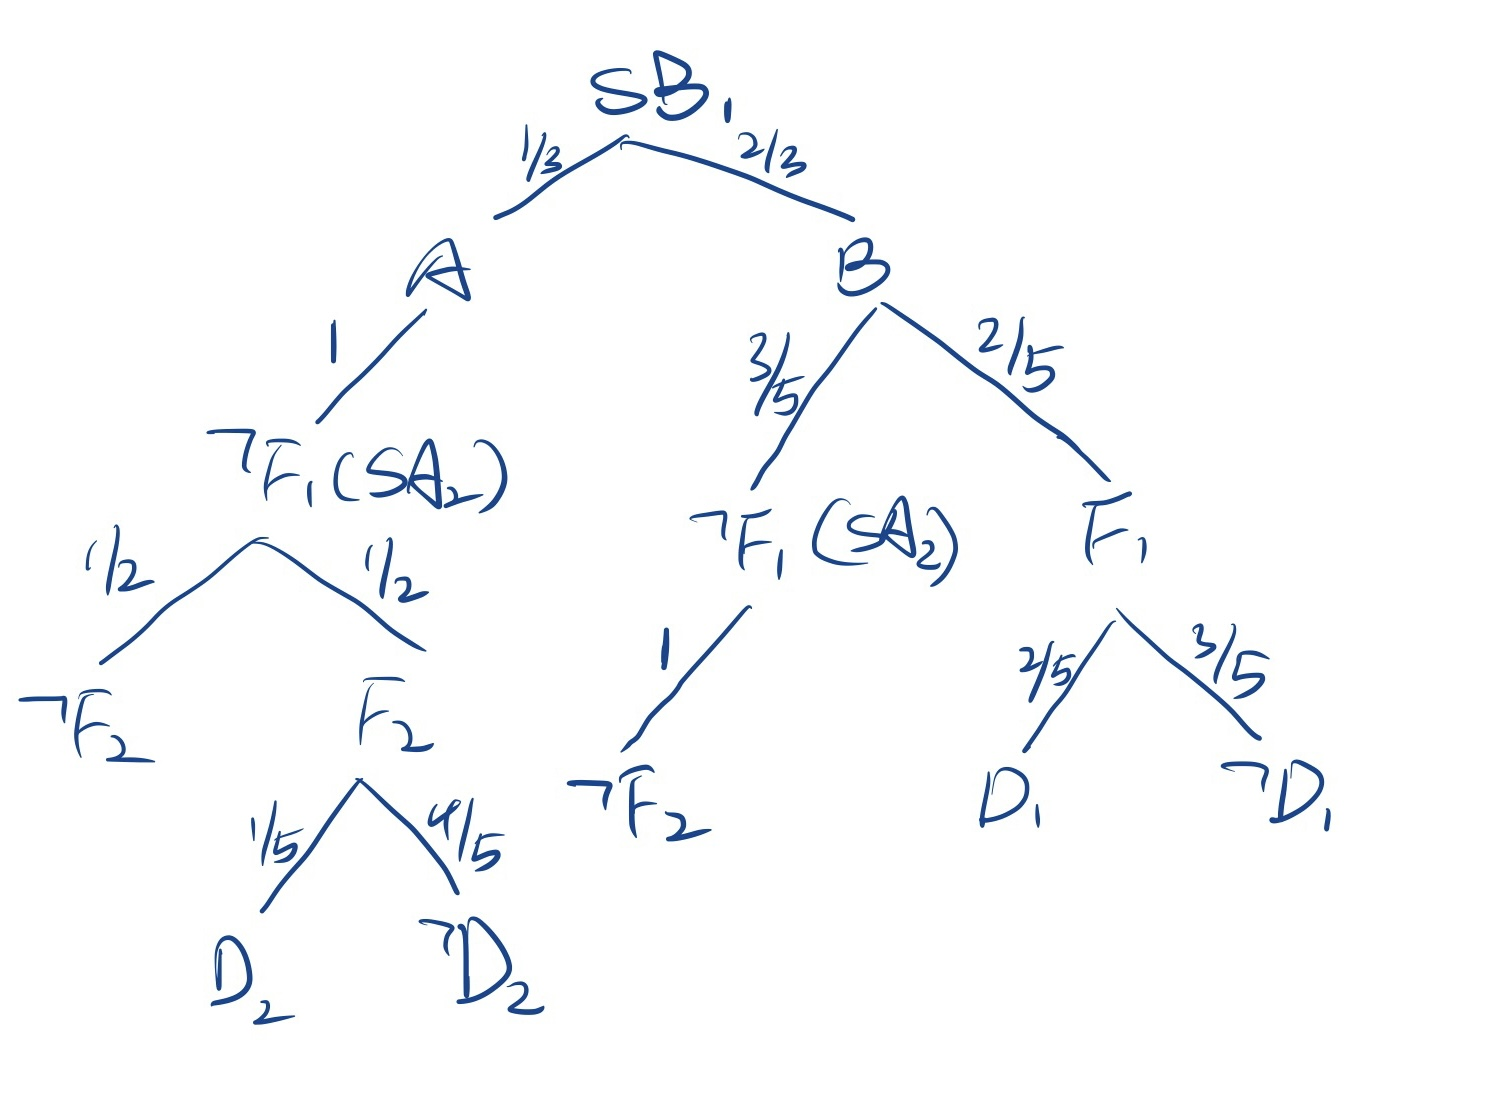
\includegraphics[width=90mm]{images/image1.jpg}
            \caption{Decision Tree \label{overflow}}
            \end{figure}
            Let $X$ denote the value that Oscar earned up to the end of day 2. Let $\mathbb{S}$ denote the state space of $X$. 
            \\$\mathbb{S}$ has only $6$ states i.e. $\mathbb{S} = \{s_1, s_2, s_3, s_4, s_5, s_6\}$, where 
            \begin{align*}
                s_1 &:= Val(A \land \neg F_1 \land \neg F_2) = -19
                \\ s_2 &:= Val(A \land \neg F_1 \land F_2 \land D_1) = -9
                \\ s_3 &:= Val(A \land \neg F_1 \land F_2 \land \neg D_2) = 51
                \\ s_4 &:= Val(B \land \neg F_1 \land \neg F_2) = -19
                \\ s_5 &:= Val(B \land F_1 \land D_1) = -3
                \\ s_6 &:= Val(B \land F_1 \land \neg D_1) = 57
            \end{align*}
            Given that:
            
        \begin{align*}
        &P[A \land \neg F_1 \land \neg F_2] = P[X=s_1]= \frac{1}{3} \times 1 \times \frac{1}{2} = \frac{1}{6}
        \\ &P[A \land \neg F_1 \land F_2 \land D_2] = P[X=s_2] = \frac{1}{3} \times \frac{1}{2} \times \frac{1}{5} = \frac{1}{30}
        \\ &P[A \land \neg F_1 \land F_2 \land \neg D_2] = P[X=s_3] = \frac{1}{3} \times 1 \times \frac{1}{2} \times \frac{4}{5} = \frac{4}{30} 
        \\ &P[B \land \neg F_1 \land \neg F_2] = P[X=s_4] = \frac{2}{3} \times \frac{3}{5} \times 1 = \frac{6}{15}
        \\ &P[B \land F_1 \land D_1] = P[X=s_5] = \frac{2}{3} \times \frac{2}{5} \times \frac{2}{5} = \frac{8}{75}
        \\ &P[B \land F_1 \land \neg D_1] = P[X=s_6] = \frac{2}{3} \times \frac{2}{5} \times \frac{3}{5} = \frac{12}{75}
        \end{align*}
    
        \begin{align*}
            \mathbb{E}(X) 
            & =  P[X=s_1] \times (-19) + P[X=s_2] \times (-9) + 
           P[X=s_3] \times 51 
           \\ &+ P[X=s_4] \times (-19) + P[X=s_5] \times (-3) + P[X=s_6] \times 57
           \\ & = \frac{1}{6} \times (-19) + \frac{1}{30} \times (-9) + \frac{4}{30} \times 51 + \frac{6}{15} \times (-19) + \frac{8}{75} \times (-3) + \frac{12}{75} \times (57)
           \\ & = \frac{68}{15}
       \end{align*}
    
        
    \end{enumerate}
    
    
\end{enumerate}
\end{document}
